% Chapter 1
\setstretch{1}
\chapter{Introduction: A Better Interactive Design Method}\thispagestyle{empty} % Main chapter title

\label{Chapter1} % For referencing the chapter elsewhere, use \ref{Chapter1} 

\lhead{Chapter 1. \emph{A Better Interactive Design Method}} % This is for the header on each page - perhaps a shortened title
\setstretch{2}
%----------------------------------------------------------------------------------------
%	Abstract
%----------------------------------------------------------------------------------------
\section{Designing Software to Power Experience}
Software is eating the world. Software is all around us. Software is a conversation and software is a dictator.Computers manage an element of almost every interaction in North America, from bus schedules to e-mail to bank reporting, to entertainment media of every stripe. In 2014, much of our work and the majority of our promotion lives in the digital world, and artistic works are no exception. Computers supply mechanisms to automate and extend our ability to speak in repeatable patterns \parencite{glanville}, returning a multiplier effect on even the most complex works.

The effective use of these tools requires a specific skill set, as unique as the skill set of using a paintbrush, yet without the consistency: digital tools change all the time. How can a designer be sure any given tool will be useful to anyone, once it's made?

This paper addresses how we might bring a new kind of old conversation to software development, derived from artist-led technical collaboration, to community prototype testing, to a standalone product. That result is a tool for making interactive video art into an open format.

\section{Interaction and Presentation in Game Design}
In the context of this paper, my frame for the term "art" is digital games as interactive experience. In this case, technology design and game design must be considered together, in that the design of an experience is dependent on its technology.

That games are art, or can be art, has been popularly contested. Famously, in 2005, Roger Ebert took the position that games could never be art \parencite{ebert1}. He recanted this statement in 2010, with a public admission of bullheadedness and a confession that he simply did not wish to engage with games as a form \parencite{ebert2}. The debate has been reasonably settled, to my mind, with the rise of conferences such as Different Games NYC and Indiecade that foster expansions to an art form with experiences at all investment levels to explore a variety of human experience. Manufacturing those experiences within a game is a challenging task, not least because game production can be expensive and thus closed. 

Games, particularly the subset of video games known as triple-A or AAA, are expensive to make and require a team of people to produce. Triple-A is the term used to refer to major popular game releases by large studios, products such as \textit{Titanfall} (2014) or \textit{Assassin's Creed}. This can be seen as restricting the degree to which the stories these experiences communicate can be personal. A large budget requires a large payback. While there are counter-examples, many triple-A games need to be able to make back their production budget, which restricts their intended audience to those who will pay to play, an audience apparently percieved at the corporate level to be overwhelmingly white, cis-gendered males. Games as self-aware  as 2013's \textit{Saint's Row 4}, \parencite{saintsrow} are few and far between. \textit{SR4} cleverly presents balanced gender roles and skin colours, yet still emphasizes that violence and exploration are the main interaction system of its world. Despite growing interest and participation in gaming by female or queer identified players, these perspectives remain almost uniformly absent and underrepresented in Triple-A.

This creates a design challenge: How to encourage a different game-making perspective entirely?

There are resistances: Unity, a 3D action engine, has been used to produce \textit{Gone Home} \parencite{fullbrightco}, a work about a missing family mainly told through examining objects and listening to music. More narrowly, the Twine engine is designed to provide branched, highly-stylized text narrative to a web browser and it has been adopted by a user base interested in telling detailed stories that are highly personal - the sort of work that cannot always be addressed by games with a bigger budget. The engine sets the form of the interaction but not the content presented by the interaction.

Artist-led collaboration is one possible approach, especially if it is followed by writing an engine to reproduce those working practices and simplify them for new users. 
 
\section{Initial Approach}
\subsection{Artist-Led Collaboration with Hannah Epstein and game::play Lab}
The initial code of screenPerfect came about as part of a collaborative research and development project in OCADu's game:play lab. The research looked to produce a vision of how dual and multi-screen game artworks might work going forward. The original software powered a game called psXXYborg \parencite{psxxyborg}, made by Hannah Epstein under the supervision of Emma Westecott. From there, I became curious as to how we could transform the engine software to include game-editing tools, to encourage a wider range of video artists to use the software. This became the basis of the initial portion of my thesis work, the screenPerfect engine.

The idea following on the engine itself is that it should be able to be installed and maintained using internet technologies for simple inter-device communication, while still being able to disconnect and install the work in a variety of specialized contexts that are free of conventional resources, such as access to the broader communications network implied by the term "internet."

\subsection{Software Development}
The initial software of this project was developed as a response to the lack of privacy and commercial control of various shared media sources online. 

Part of the motivation for this engine is that commercial engines tend to prioritise commercial distribution and mass experience, whereas artist installations tend to prioritise the direct experience of a specific work at a specific time. Although there are commercial FMV engines, they do not permit easy access to multi-screen synchronisation and cannot be accessed offline. This meant that presenting the works developed using these systems meant agreeing to advertising, or to sign up for an account with the company, rather than being able to turn on an appliance and serve an art work.

This technology is built to be served offline using technologies more commonly seen online. This is made possible through use of the Node.JS software framework, which, combined with Google's Chrome browser (a variant of webkit), permits web applications to be used the same way people have historically used desktop variants. The benefit of this is that web technologies are straightforward to use to connect devices, where local installations traditionally rely on the resources of only their specific machine. The code of screenPerfect is written wholly in javascript via the Node.JS software framework.

No Jam 2 featured both an editing segment and a re-architected version of screenPerfect that uses Bento Box-Miso's Daimio dataflow language \parencite{daimio}, designed mainly for open use on the internet. After the jam, the games were collected and screenPerfect was forked to become two separate engines. The original engine was retained for displaying works to that point. A new engine called iV was created by Bento Box-Miso to promote ease of access for Dames Making Games, a feminist community group run at Miso by the same developers who worked on the engine.

The toolset can then be released for new users to create new works by packaging the application to run on a USB stick, conceptually similar to game cartridges from the 1990s (Figure 1.1). This means that artists will be able to install and display their own games independent of any central server, free of what the technician might decide is the context of the work. This is intentional and has been included to help resolve many of the issues inherent in the storage and display of networked digital artworks. By having an independent, repeatable system that lives on a single SD card and uses identical, widely-available, afforable hardware, it becomes straightforward to both archive and recall works, as each version can be stored and then loaded independently, if required.

This reliable installation mechanism also permits the display of completed works even in remote contexts – a forest, for example, or a desert (Figure 1.2). This is distinct from other systems in that it is built using contemporary technologies but also in that it is built with an eye to permanent, disconnected installations that rely on contained software and simple, contemporary script languages, rather than on translations of preexisting software such as Java.

\begin{figure}[!ht]
\centering
  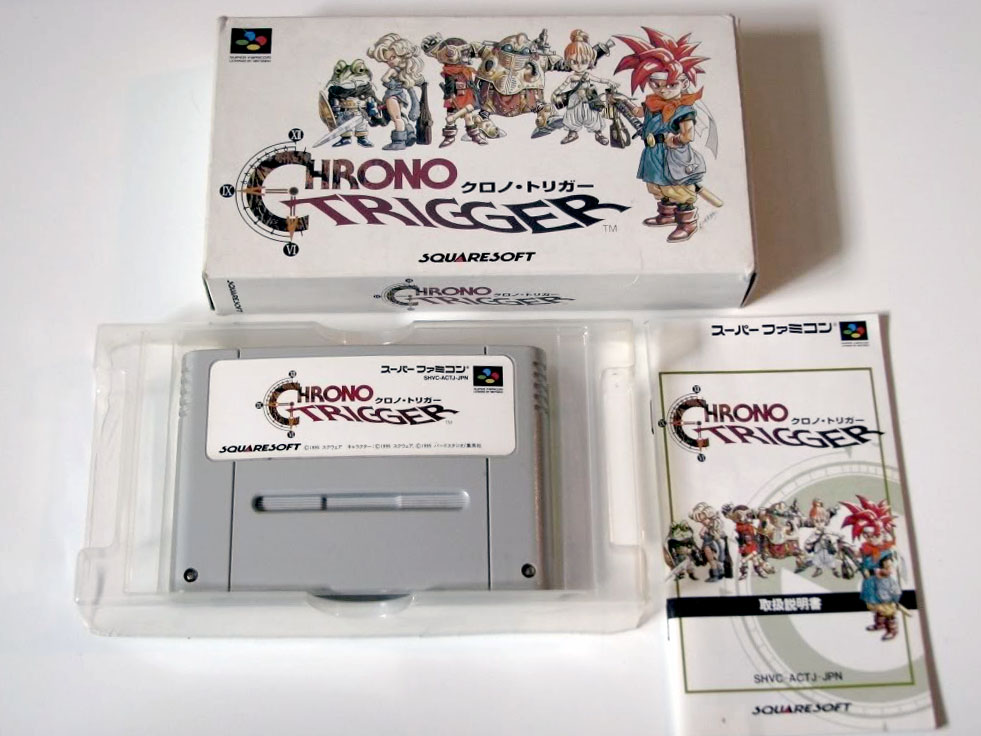
\includegraphics[width=0.5\textwidth]{gamecart}
 \caption{SNES Game Cartridge, 1995}
\end{figure}

\section{Community Based Prototype Design with Dames Making Games and Bento Box-Miso: Overcoming Imposter Syndrome}

In order to refine screenPerfect to a tool for popular use, rather than a specific engine requiring a technician, I partnered with game::play Lab, Dames Making Games and Bento Box-Miso. We collaboratively organized a game jam - a type of design charette, intended to produce demonstratable games in a compressed window of time - that would both test the tool and introduce new game makers to the possibilities of FMV.

The critical theory that underlies this practice is a combination of French poststructuralism - H\'{e}l\`{e}ne Cixous in particular - and contemporary writing on video games and the history of women in technology. By producing the software and content with the input of a local feminist collective, Dames Making Games (\url{http://www.dmg.to}), and as part of a wider feminist research network (SSHRC-funded Feminists in Games (\url{http://www.feministsingames.com})), I have grounded the work in a social justice driven practice which encourages women to take part in their own lives by learning how to interact with machines and communicate with the broader world.

Dames Making Games' mission is to organize women-focused game jams and support women gamemakers. New, straightforward game-making tools provided with the intent to reduce the barriers to producing a game or interactive work, shifting the focus from frustration with game engine's normal assumptions about design to an emphasis on the user's content. By removing barriers such as the requirement for complex scripting, we hope to expand the diversity of experience that can be expressed by new game-makers. 

This is an explicitly feminist goal, derived in part from H\'{e}l\`{e}ne Cixous' "Laugh of the Medusa," in which she describes the necessity of women writing to produce themselves. Cixous' concept describes a space where women required to write, even using imperfect language or tools, least they be written out by the dominant voices that surround them. The \textit{écriture féminine} is also about insists on rebellion with a sense of play, which I find resonant with the practice of feminist, open game jams for learning and self-expression \parencite{cixous}. 

The embodiment emphasized by Cixous is tied to display of personal narrative. Whilst many game works wish to leave the body behind, or optimize it to an ideal form in a play avatar, almost all of the games produced at NoJam 2 had a strong association to the body. Max Lander's \textit{PornGame} explored what it means for a computer to desire interaction, in a sexual sense. Brittney Oberfeld's \textit{OM} explored the embodiment of consciousness and a desire to "slow down," Kate Whyte and Kara Stone's \textit{Cyborg Goddess} presented an adventure through the loss of a leg and the replacement with supplementary systems to become a cyborg or a goddess. \textit{Grimoire}, by Katie Foster and Mikayla Carson, detailed a woman's descent into madness following the discovery of an ancient text.

This seems to be a refraction of the ability of code to make the written tangible.  When you touch a screen, writing – interpreted or compiled – controls what happens next. In this context, the \textit{écriture féminine}can involve a physical change in the environment. The ideas are vividly expressed in relationship mainly to sexuality but desire runs deeper than that: desire can include the desire for agency, for authority over oneself and one's life, or to be seen as competent even by oneself. In this Cixous provides a resistance to imposter syndrome.

Imposter syndrome is common in technological fields, where women form a small percentage of professional game developers - some estimate as low as 4\%, where IGDA numbered 9\% in the last public study released - in 2007 \cite{igda}. Despite this, women consist of a larger percentage of the gameplaying public. The ESA states that women form at least 31\% of the game-buying public, almost double the number of teenaged males \parencite{esa}. The gap between developer and player implies that it is important to provide a way to encourage women to express themselves in this new game form, least women be seen as an alien construct within technological fields. 

\section{Prototype Development: Hardware Installation and Display}

The final section of this paper addresses thoughts on hardware installation and the display of digital works. digital works are difficult to maintain and display because they frequently rely on external systems, such as the public internet, to be consistent and always available. This has proven to be challenging in practice. Rather than relying on a central remote server, in this chapter I address reasons to provide solid hardware in an appliance format for application display, rather than relying on external resources that may or may not be available. 

This chapter is perhaps the most politically informed, as Chapter 2 is informed by the idea that artists should be permitted control over their works and encouraged to produce works using contemporary media. The production of affordable, repeatable installations based on the not-for-profit Raspberry Pi platform means that artists who have participated in web application game jams can then own their own works in the form of common memory and display those works with minimal personal outlay on hardware. This section also asks that we consider our reliance on major internet corporations and how we might separate the computers we use to produce art from the computers we use to serve that art to our audience.

Chapter 4 also presents a number of display scenarios that make use of interesting contexts that do not have ready access to major power or consistent internet. It also presents the idea that the context of the display can extend the value of the work in meaningful ways.

\clearpage
\thispagestyle{fancy}\lhead{Chapter 1. \emph{A Better Time-Based Installation}} 
\begin{figure}[!ht]
 \centering
  \includegraphics[width=\textwidth]{DevelopmentFramework}
  \caption{A method for realizing artist-led technical collaboration.}
\end{figure}
\newpage

